% ==============================================================================
% PG - Sophie Dilhon
% Capítulo 4 - Projeto Arquitetural e Implementação
% ==============================================================================
\chapter{Projeto Arquitetural e Implementação}
\label{chap-projeto}

\section{Modelos FrameWeb}
\label{sec-projeto-frameweb}

Nessa seção são apresentados os modelos FrameWeb, construídos na fase de Projeto Arquitetural
do SCAP, com o objetivo de guiar a fase de implementação do sistema.

\subsection{Modelo de Entidades}
\label{subsec-frameweb-entidades}
O modelo de entidades de FrameWeb é um diagrama de classes UML que representam
os objetos de domínio do problema e seu mapeamento para a persistência no banco de dados
relacional. A partir dele são implementadas as classes da camada de domínio~\cite{souza:2007}.

A Figura \ref{fig-modelo-entidades} apresenta o modelo de entidades do SCAP. O modelo foi feito
a partir do diagrama de classes mostrado anteriormente, com adaptações para a plataforma 
escolhida para a implementação do sistema, dessa forma são apresentados os tipos
de cada propriedade. A Figura \ref{fig-modelo-entidades-enum} apresenta
os tipos enumerados do modelo de entidades do SCAP.

\sophie{Adicionar not null e ver se precisa adicionar se é privado ou público}
\begin{figure}
    \centering
    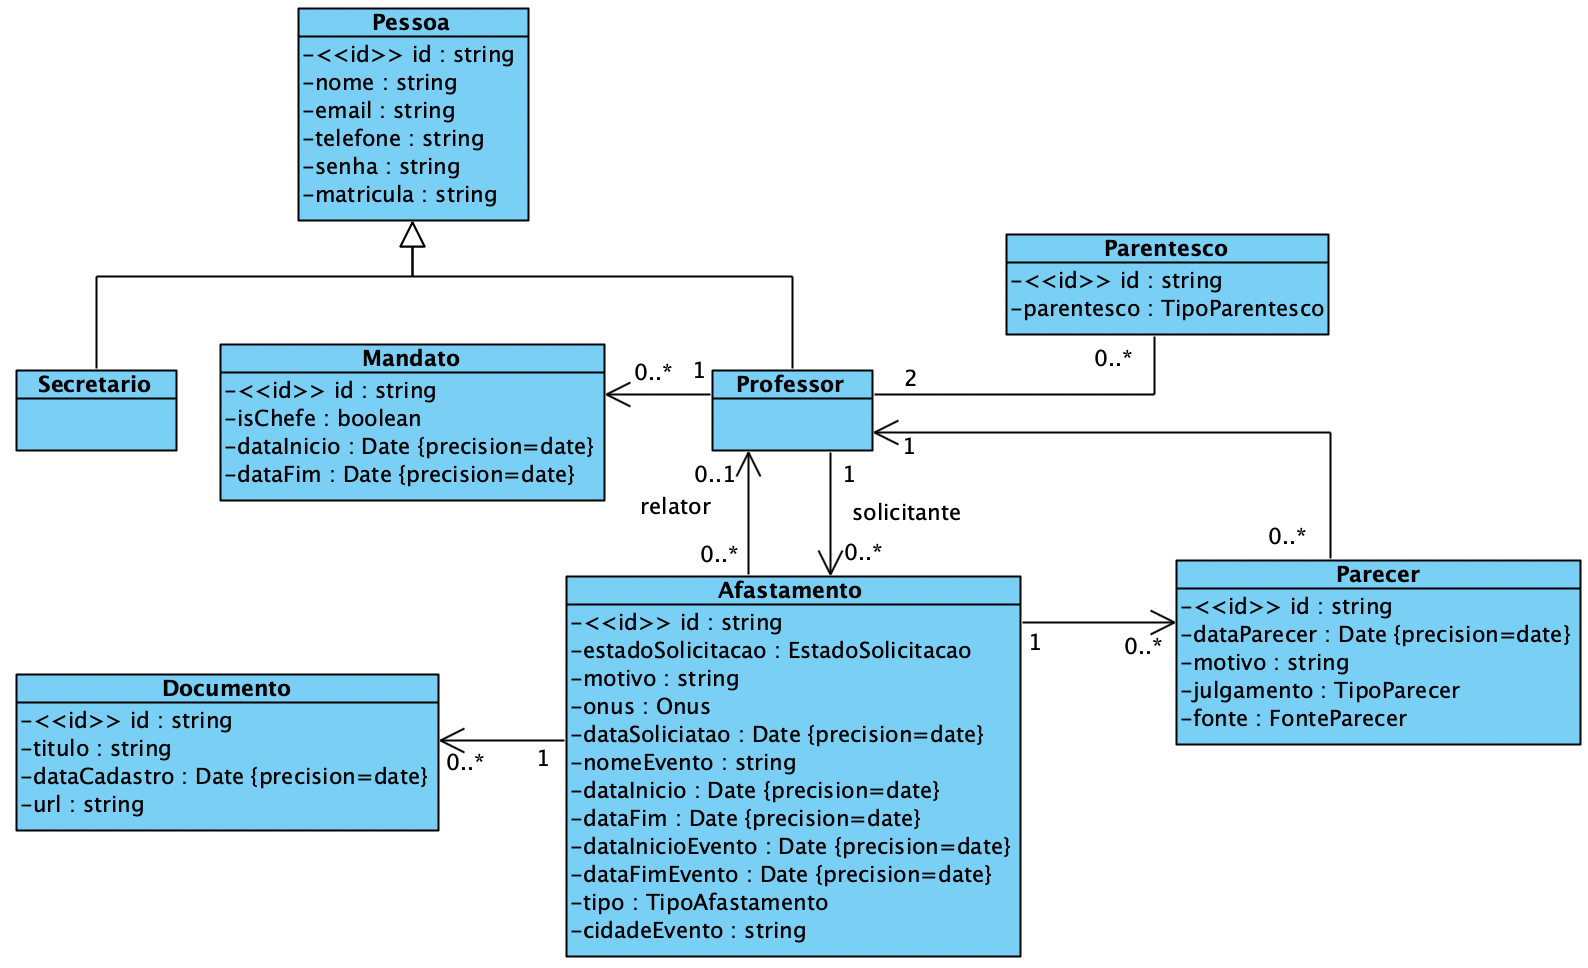
\includegraphics[width=1\textwidth]{figuras/fig-modelo-entidades.png}
    \caption{Modelo de Entidades do SCAP.}
    \label{fig-modelo-entidades}
\end{figure}

\begin{figure}
    \centering
    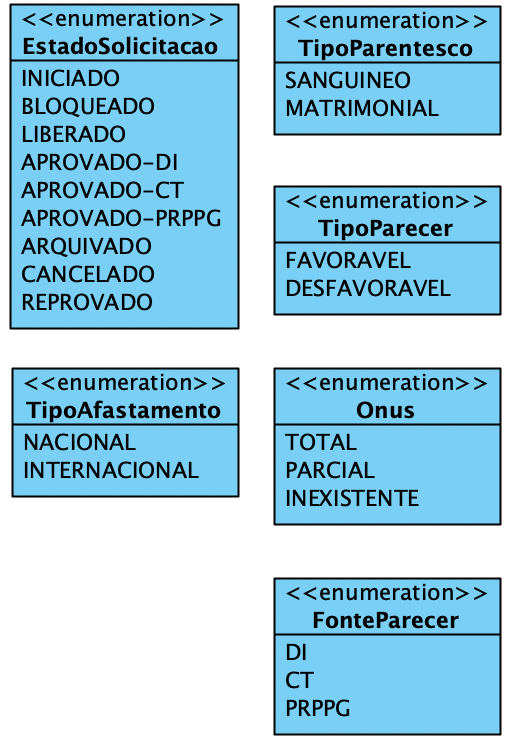
\includegraphics[width=0.5\textwidth]{figuras/fig-modelo-entidades-enum.png}
    \caption{Tipos Enumerados do Modelo de Entidades do SCAP.}
    \label{fig-modelo-entidades-enum}
\end{figure}


\subsection{Modelo de Persistência}
\label{subsec-frameweb-persistencia}


\subsection{Modelo de Navegação}
\label{subsec-frameweb-navegacao}


\subsection{Modelo de Aplicação}
\label{subsec-frameweb-aplicacao}